
\documentclass[11pt]{article}

% math packages
\usepackage{mathtools}
\usepackage{amsmath}
\usepackage{amssymb}    % Math symbols such as \mathbb
\usepackage{amsthm}
\usepackage{pgfplots}   % plots

% other packages
\usepackage{graphicx}
\graphicspath{ {../assets/} }
\usepackage{enumitem}
\usepackage[a4paper, total={6in, 8in}]{geometry}
\usepackage{hyperref}

% proper inline math display, adjust height for symbols like \sum
\everymath{\displaystyle}

% define tags for math use..
\theoremstyle{plain}% default
\newtheorem{theorem}{Theorem}[section]
\newtheorem{corollary}{Corollary}[theorem]

\theoremstyle{definition}
\newtheorem{defn}{Definition}[section]
\newtheorem{exmp}{Example}[section]

\theoremstyle{remark}
\newtheorem*{rem}{Remark}
\newtheorem*{note}{Note}
\newtheorem{case}{Case}

% Gives begin{solution} same formating as \begin{proof}
\newenvironment{solution}
  {\begin{proof}[Solution]}
  {\end{proof}}


%running fraction with slash - requires math mode.
\newcommand*\rfrac[2]{{}^{#1}\!/_{#2}}
%shortcut to mathbb
\newcommand{\N}{\mathbb{N}}
\newcommand{\R}{\mathbb{R}}
\newcommand{\I}{\mathbb{I}}
% color highlighting
\newcommand{\hilight}[1]{\colorbox{yellow}{#1}}


\title{MAT237 Problem Sets}
\author{Mark Wang}

% begin document
\begin{document}

% title page
\maketitle


% problem set 1
\section*{Problem Set 1}


\subsection*{Definitions}

\begin{defn}
  \label{union}
  Let S be a set and choose 2 sets $A, B \subseteq S$. The \textbf{union} of A and B is
  \[
    A\cup B = \left\{ x\in S | \quad x\in A \lor x\in B \right\}
  \]
  \[
    \bigcup_{i\in \I} A_i = \left\{ x\in S | \quad \exists i\in I, x\in A_i\right\}
  \]
\end{defn}

\begin{defn}
  \label{intersection}
  Let S be a set and choose 2 sets $A, B \subseteq S$. The \textbf{intersection} of A and B is
  \[
    A\cap B = \left\{ x\in S| \quad x\in A \land x\in B \right\}
  \]
  \[
    \bigcap_{i\in\I} A_i = \left\{ x\in S | \quad \forall i \in I, x\in A_i \right\}
  \]
\end{defn}

\begin{defn}
  \label{setcomplement}
  If $A\subseteq S$, then the \textbf{complement} of A with respect to S is all elements which are not in A, that is
  \[
    A^c = \{ x\in S: x\not\in A \}
  \]
\end{defn}

\begin{defn}
  \label{function}
  Given 2 sets A, B, a \textbf{function} $f: A\to B$ is a map which assigns to every point in A a unique point of B, that is
  \[
    f: a \mapsto f(a), \text{ where } a\in A, f(a)\in B
  \]
\end{defn}

\begin{defn}
  \label{image and preimage}
  Let $f: A\to B$ be a function.
  \begin{enumerate}
    \item If $U \subseteq A$, then we define the \textbf{image} of $U$ to be
    \[
      f(U) = \left\{ y\in B: \exists x\in U, f(x) = y\right\} = \left\{ f(x): x\in U\right\}
    \]

    \item If $V\subseteq B$ we define the \textbf{pre-image} of $V$ to be
    \[
      f^{-1}(V) = \left\{ x\in A: f(x) \in V\right\}
    \]
    \begin{rem}
      Note $U,V$ are sets, not variable.
    \end{rem}
  \end{enumerate}
\end{defn}

\begin{defn}
  \label{jectivity}
  Let $f: A \to B$ be a function. We say that
  \begin{enumerate}
    \item f is \textbf{injective} if whenever $f(x) = f(y)$ then $x=y$
    \item f is \textbf{surjective} if for every $y\in B$ there exists $x\in A$ such that $f(x) = y$
    \item f is \textbf{bijective} if f is both injective and surjective
  \end{enumerate}

  \begin{rem}
    Testing injectivity by using the horizontal line test in $\R^2$: An injective function is one whose graph that never intersect any horizontal line twice. Test surjectivity by ensuring that every horizontal line in the domain is crossed at least once by the graph.
  \end{rem}
\end{defn}

\newpage

\subsection*{Problem 1}
Let $A\subseteq S$ and $B\subseteq S$. Prove each of the following statements \\
\begin{enumerate}
  \item $A\subseteq B$ if and only if $A\cup B = B$
    %% problem 1.1
    \begin{proof}
      $ $\newline
      \textbf{(if)} Given $A\cup B = B$. Proof by contradiction (always assume the opposite of the conclusion is true). Assume $A\not\subseteq B$, which means $\exists x \in A, x \not\in B$. Also $x\in A\cup B$. Because $A\cup B = B$, then $x\in B$. This contradicts with $x\not\in B$. Therefore $A\subseteq B$ if $A\cup B = B$ \\
      \textbf{(only if)}  $A\cup B$ means $\exists x\in S, x\in A \lor x\in B$. Because given $A\subseteq B$, which means if $x\in A$ then $x\in B$, $\exists x\in S, x\in A \lor x\in B$ is equivalent to $\exists x\in S, x\in B$, which is the definition of B
    \end{proof}
    %% end problem 1.1
  \item $A^{c}\subseteq B$ if and only if $A\cup B = S$
    %% problem 1.2
    \begin{proof}
      $ $\newline
      \textbf{(if)} Given $A\cup B = S$, then if $x\in S$, then $x\in A \lor x\in B$. Use proof by contradiction. Assume $A^{c}\not\subseteq B$, let $x \in S$ such that $x \in A^c$, then $x\not\in B$. Therefore $\exists x\in S, x\not\in A \land x\not\in B$. This contradicts with the first sentence of the proof. Therefore $A\cup B = S \Rightarrow A^{c}\subseteq B$ \\
      \textbf{(only if)} Given $A^{c}\subseteq B$. Proof by contradiction. Assume $\exists x \in S, x\not\in A\cup B$, then $x\not\in A \lor x\not\in B$. $x\not\in A$ is equivalent to $x\in A^{c}$, which implies $x\in B$ by $A^{c}\subseteq B$. Contradiction arises as $x$ cannot be in both $B$ and not in $B$.
    %% end problem 1.2
    \end{proof}

  \item $A\subseteq B$ if and only if $B^{c}\subseteq A^{c}$
    %% problem 1.3
    \begin{proof}
      $ $\newline
      \textbf{(if)}
      Given $B^{c}\subseteq A^{c}$. Proof by contradiction. Assume $A \not\subseteq B$. Then $\exists x\in A, x \not\in B$. $x\not\in B$ is equivalent to $x\in B^c$, then by  $B^{c}\subseteq A^{c}$, $x \in A^c$. Contradiction happens when $x\in A$ and $x\in A^c$. \\
      \textbf{(only if)}
      Given $A\subseteq B$. Proof by contradiction. Assume $B^{c}\not\subseteq A^{c}$, then $\exists x\in S, x\in B^c \Rightarrow x\not\in A^c$. Then $x\not\in B \Rightarrow x\in A$, and by $a\subseteq B$, $x\not\in B \Rightarrow x\in B$. Contradiction arises
    %% end problem 1.3
    \end{proof}

  \item $A\subseteq B^{c}$ if and only if $A\cup B = \emptyset$
    %% problem 1.4
    \begin{proof}
      $ $\newline
      \textbf{(if)}
      Assume $A\cup B = \emptyset$. Then $A=B=\emptyset$. Then $B^c = S$. Therefore, $\emptyset = A \subseteq B^c = S$ \\
      \textbf{(only if)}
      Assume $A\subseteq B^{c}$, then
      \hilight{how do you prove this...}
    %% end problem 1.4
  \end{proof}
\end{enumerate}


\subsection*{Problem 2}
Let A, B, and C be subsets of S. Show that if $A\subseteq B$ and $B\subseteq C$, then $A\subseteq C$.

\begin{proof}
  $ $\\
  Given $A\subseteq B$ and $B\subseteq C$. Let $x\in S, x\in A$, then $x\in B$ by $A\subseteq B$. Then $x\in C$ by $B\subseteq C$. Therefore, $x\in A \Rightarrow x\in C$, which means $A\subseteq C$.
\end{proof}


\subsection*{Problem 3}
Let $f:A\to B$ be a map of sets, and let $\left\{X_{i}\right\}_{i\in I}$ be an indexed collection of subsets of A.

\begin{enumerate}
  \item Prove that $f\left(\bigcup_{i\in I} X_{i}\right) = \bigcup_{i\in I} f(X_{i})$
    % problem 3.1
    \begin{proof}
      $ $\\
      \[
      \begin{split}
        LHS &= \left\{ y \in B: \exists i\in \I, x\in X_i \text{ and } f(x)=y\right\} \\
        &=  \left\{ y \in B: \exists i\in \I, y\in f(X_i)\right\} \\
        &= RHS
      \end{split}
      \]
    \end{proof}

    \begin{rem}
      Refer to \hyperref[image and preimage]{definition~\eqref{image and preimage}} and \hyperref[union]{definition~\eqref{union}} for proof. Think both forward and backward to find a common claim.
    \end{rem}
    % end problem 3.1
  \item Prove that $f\left(\bigcap_{i\in I} X_{i}\right) \subset \bigcap_{i\in I} f(X_{i})$
    % problem 3.2
    \begin{rem}
      Intuitively speaking, non-injective function will follow this claim.
    \end{rem}
    \begin{proof}
      $ $\\
      \[
      \begin{align}
        LHS &= \left\{ y \in B: \forall i\in \I, x\in X_i \text{ and } f(x)=y\right\} \\
        RHS &= \left\{ y \in B: \forall i\in \I, y\in f(X_i)\right\} \\
      \end{align}
      \]
      \hilight{dunno how to prove this...}
    \end{proof}
    % end problem 3.2
  \item When does equality of sets hold in the above part? \\
    % problem 3.3
    Prove $f\left(\bigcap_{i\in \I} X_{i}\right) = \bigcap_{i\in I} f(X_{i})$ if and only if f is injective

    \begin{proof}
      $ $\\
      ($\Leftarrow$) \\
      Assume f is injective. Let $y \in \bigcap_{i\in \I} f(X_i)$. This means $y \in f(X_i)$ for all $i \in \I$, which means $\forall i \in\I, \exists x_i \in X: f(x_i) = y$. Since f is injective, $f(x_i) = y$ for all $i \in\I$ (the preimage is just one x) means $x_1 = \dots = x_i = \dots = x$. So $x\in\bigcap_{i\in\I}X_i$. So $y=f(x)\in f(\bigcap_{i \in\I} X_i)$ \\
      ($\Rightarrow$) \\
      Assume $f\left(\bigcap_{i\in \I} X_{i}\right) = \bigcap_{i\in I} f(X_{i})$. Think about what it means for f to not be injective --- when $x\neq y, f(x) = f(y)$
      \[
        \emptyset = f(\emptyset) = f(\{x\}\cap\{y\}) = f(\{x\})\cap f(\{y\}) = f(\{x\})
      \]
      Thus there is no such $x,y$. This is a contradiction.
    \end{proof}

    \hilight{dont really understand this.}
    % end problem 3.3
\end{enumerate}

\subsection*{Problem 4}
Consider the map $f: \R \to \R, x \mapsto \sin(x)$

\begin{enumerate}
  \item Find the image of the set $[0,\pi]$; that is, determine $I = f([0,\pi])$. \\
  % problem 4.1
  \[
    I = f([0,\pi]) = \{f(x): x \in [0, \pi]\} = [0, 1]
  \]
  % end problem 4.1
  \item Let $I$ be as in the previous question. Determine the preimage $f^{-1}(I)$. \\
  % problem 4.2
  \[
    f^{-1}(I) = \{ x \in R: f(x) \in [0, \pi]\} = \bigcup_{i\in\I} [2\pi i, 2\pi(i+1)]
  \]
  % end problem 4.2

  \begin{rem}
    Use \hyperref[image and preimage][definition~\eqref{image and preimage} to solve the problem
  \end{rem}
\end{enumerate}


\subsection*{Problem 5}
Consider the function $F: \R^2 \to \R, (x,y) \mapsto y - x^2$

\begin{enumerate}
  \item Graph the set $F^{-1}(0)$ in $\R^2$ \\
  \[
    \begin{split}
      F^{-1}(0) &= \{ (x, y)\in \R^2: F((x, y)) = 0 \} \\
      &= \{ (x, y)\in \R^2: y - x^2 = 0 \}
    \end{split}
  \]
  \begin{center}
    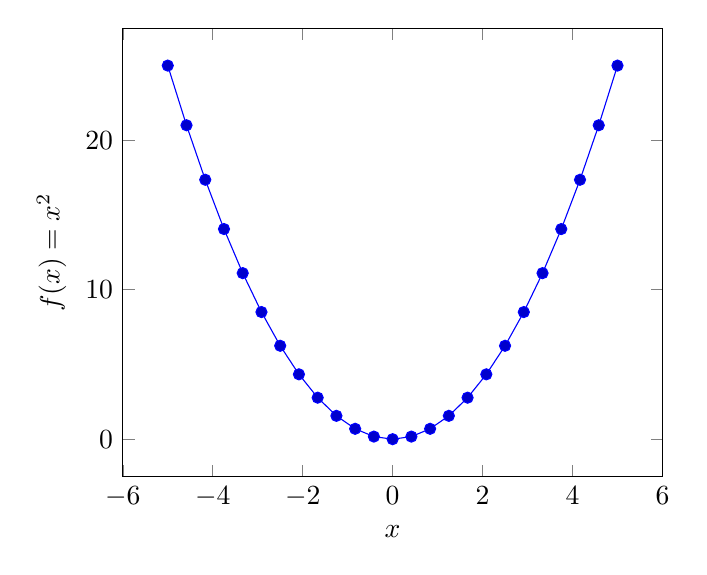
\begin{tikzpicture}
      \begin{axis}[
        xlabel=$x$,
        ylabel={$f(x) = x^2 $}
      ]
        \addplot {x^2};
      \end{axis}
    \end{tikzpicture}
  \end{center}
  \item More generally, if $c \in \R$ is any real number, what does the set $F^{-1}(c)$ look like?
  \[
    \begin{split}
      F^{-1}(c) &= \{ (x, y)\in \R^2: F((x, y)) = c \} \\
      &= \{ (x, y)\in \R^2: y - x^2 = c \}
    \end{split}
  \]
  The plot would be $y=x^2$ that translate vertically $c$ units.
\end{enumerate}


\subsection*{Problem 6}
Let $I$ be an index for a collection of subsets $A_{i}\subseteq S, i \in I$. Show that for every $k \in I$, $\bigcap_{i\in I}A_{i}\subseteq A_{k}$

\begin{solution}
  $ $\\
  Assume $\bigcap_{i\in I}A_{i}\subseteq A_{k}$. Let $a\in \bigcap_{i\in I}A_{i}$, then $a\in \{ x\in S: \forall i\in I, x\in A_i\}$. Therefore for every $k\in I, a \in A_k$ by previous definition. This proves $\bigcap_{i\in I}A_{i}\subseteq A_{k}$.
\end{proof}




\subsection*{Problem 7}
Give an example of a function $f(x) = \left( f_1(x), f_2(x) \right)$, such that neither of the component functions $f_1,f_2$ are injective, but $f$ is injective. Be sure to specify the domain of f.

\begin{solution}
  $ $\\
  Let $f_1: \R \to \R^+, x \mapsto x^2$, and $f_2: \R \to \R^+, x\mapsto x^4$. Both $f_1, f_2$ are not injective. To prove $f_1$ is not injective. Let $a_1 = 2, a_2 = -2, f_1(a_1) = 4 = f_1(a_2)$. However $a_1 \neq a_2$, $f_1$ is not injective. Same is true for $f_2$. The resulting function $f: \R \to X, x \mapsto (x^2, x^4)$ is injective.

  uhh this is wrong what is the answer
\end{solution}



\subsection*{Problem 8}
Let $f: A\to B$ be a function.

\begin{enumerate}
  \item For every $X\subseteq A$, $X \subseteq f^{-1}(f(X))$ \\
    \begin{rem}
      Recall \hyperref[image and preimage]{definition~\eqref{image and preimage}}. This question is implying that the preimage of an image contains the domain. It may exceed the size of domain.
    \end{rem}
    \begin{proof}
      $ $\\
      Assume $X \subseteq A$, so $f(X) \in B$.
      \[
        \begin{split}
          f^{-1}(f(X)) &= \{a \in A: f(a) \in f(X)\} \\
          &= \{ a\in A: \exists x\in X, f(a) = f(x)\}
        \end{split}
      \]
      \begin{note}
        Combination of definition for image and preimage
      \end{note}
      Let $x\in X$, try to get to $x\in f^{-1}(f(X)) = \{ a\in A: \exists x\in X, f(x) = f(a)\}$. $x$ satisfies $\exists x\in X, f(x) = f(x)$. Also $x\in X\subseteq A$, hence $x\in f^{-1}(f(X))$ by definition\\
    \end{proof}
  \item For every $Y\subseteq B$, $Y \supseteq f(f^{-1}(Y))$ \\
    \begin{proof}
    Assume $Y \subseteq B$, so $f^{-1}(Y) \in B$
    \[
      \begin{split}
        f(f^{-1}(Y)) &= \{ b\in B: \exists x\in f^{-1}(Y), f(x) = b \} \\
        &= \{ b\in B: \exists a\in A, f(a) \in Y \land f(a) = b\} \\
        &= \{ y\in Y: \exists a\in A, y = f(a)\}
      \end{split}
    \]
    Let $y\in f(f^{-1}(Y))$, then by definition $y\in Y$. Therefore $Y \supseteq f(f^{-1}(Y))$
    \end{proof}
  \item If $f: A\to B$ is injective, then for every $X\subseteq A$ we have $X = f^{-1}(f(X))$
  \begin{proof}
    Refer to question 1, we already proved that for every $X\subseteq A$, $X \subseteq f^{-1}(f(X))$. Just have to prove $X \supseteq f^{-1}(f(X))$ to show equality, on the condition that $f: A \to B$ is injective. Recall that $f^{-1}(f(X)) = \{ a\in A: \exists x\in X, f(a) = f(x)\} = \{ a\in A: \exists x\in X, a=x\}$ using injectivity of $f$. Let $x\in f^{-1}(f(X))$, then $x\in X$ by definition of $f^{-1}(f(X))$.
  \end{proof}}

  \item If $f:A\to B$ is surjective, then for every $Y\subseteq B$ we have $Y = f(f^{-1}(Y))$
  \begin{proof}
    Refer to question 2, we already proved that for every $Y\subseteq B$, $Y \supseteq f(f^{-1}(Y))$. Just have to prove $Y \subseteq f(f^{-1}(Y))$ to show equality, on the condition that $f:A\to B$ is surjective. Recall that $f(f^{-1}(Y)) = \{ y\in Y: \exists a\in A, y = f(a)\}$. Let $y\in Y$, then $\exists a\in A, y=f(a)$ by definition of surjectivity. This is equivalent to the set notation of $f(f^{-1}(Y))$, hence the arbitrary $y \in f(f^{-1}(Y))$. Therefore $Y \subseteq f(f^{-1}(Y))$. Also $Y \supseteq f(f^{-1}(Y))$, $Y=f(f^{-1}(Y))$ for every $X \subseteq A$.
  \end{proof}
\end{enumerate}






% end document
\end{document}
